As said in section \ref{subsubsec:Discretization} the simulations are done with the Scalar-weak order 2.0 Itô-Taylor method \cite[algorithm 8.5]{Srkk2019}. The concrete schemes that we derived for the respective types of noises are shown in equations (\ref{eq:OUSim} - \ref{eq:jacobiDiffusion}). A method for each scheme is implemented in \code{R}. All methods can be called with specific parameter choices, values for $\tau_c$ and $t_0$ as well as a temporal resolution, $\Delta t$ and starting point, $x_0$. \\Depending on the $\tau_c$, $t_0$, and $\Delta t$ the method dynamically picks the appropriate number of samples to draw for $\Delta W_k\sim\mathcal{N}\left(0,\Delta t\right)$. The methods allow for positive $\lambda_0$ and negative $A$, but recall that this only correspond to choosing between the positive and negative versions of (\ref{eq:standardStochasticForm}). If no starting point is specified the methods picks the fixed point in the stationary part of the process as the starting point; note that this of course is done with the appropriate branch of (\ref{eq:fixedPoint}) depending on the version of (\ref{eq:standardStochasticForm}), i.e. the sign of $A$. Additionally, an argument is implemented such that we can opt for stopping the process at earlier time (or later) points in time than $\tau_c$. This is useful, when we want to evaluate the models' ability to predict the tipping point based on how far from it we have samples. For details about the timing-benchmarks refer to section \ref{section:benchmark}. Specifications on hardware and software used can be found in table \ref{tab:specs}. 
\subsection{Overview of the estimation methods}
In this section, we test our methods on simulated data. The test aim to illustarte the robustness, computation efficiency and performance in terms of ARE (\ref{eq:ARE}). To perform the study for all the models and their respective methods at once, we sample with the parameters that worked for all models in figure \ref{figure:samplesFromAllDifferentModels}. That is $A = 1.5, m = 0.4, \lambda_0 = -0.2, \sigma = 0.1$, and we assumed throughout that $\nu = 1$, i.e. we do not estimate this parameter for now. According to the first-order taylor expansion, which we use in the stationary part (\ref{eq:TaylorStationary}), the true values are $\theta_{\mathrm{stationary}} = (1.095, 0.7651, 0.1)^\top$.  For the dynamic part, we simulate using $t_0 = 30$ and $\tau_c = 30$. We simulate with temporal resolutions $\Delta t = \{1/5, 1/10, 1/25, 1/100, 1/250\}$, corresponding to $N = \{150, 300, 750, 3000, 7500\}$ number of samples in each part of the process. For each value of $N$ we run the simulations and estimation $M = 50$ times and record the median ARE for each parameter. In addition, we calculate the median run-time for each method. In both cases we use the median due to it being more robust against outliers than the mean. Furthermore, due to the possibility of extreme samples for small $N$; we implement a \code{trycatch} suc that the program fails gracefully, if estimation fail for a model on a specific sample. For each run in the simulation all the models are simulated with the same realizations of the brownian motion; if one model fails the all models are re-run using a new seed. The optimizers are initialized at random points where each coordinate can deviate up to $\pm 10\%$ at random from the true values; this is done by sampling three uniform variables according to $U\sim\mathrm{Unif}(0.9, 1.1)$ and multiplying them with the true values.
As convergence criterion for the likelihood-based methods we use a relative tolerence of $\code{sqrt(.Machine\$double.eps)/10}\approx 1.49\cdot 10^{-9}$, while the estimation equations where an equation is numerically solved use $10^{-8}$; the standard of \code{nleqslv::nleqslv}. The likelihood based methods are the MLE and the Strang-based estimators; when there is more than one such method for a specific model, we denote it \textit{Likelihood (Alt.)}. Naturally, estimators based on the score equation or martingale estimation function based equation are estimation equation based estimators together.
\subsubsection{The stationary parts}
In the stationary parts, we run the simulations as described above and depict the median ARE as a function of sample size on a double logarithmic scale
\begin{figure}[h]
    \begin{center}
    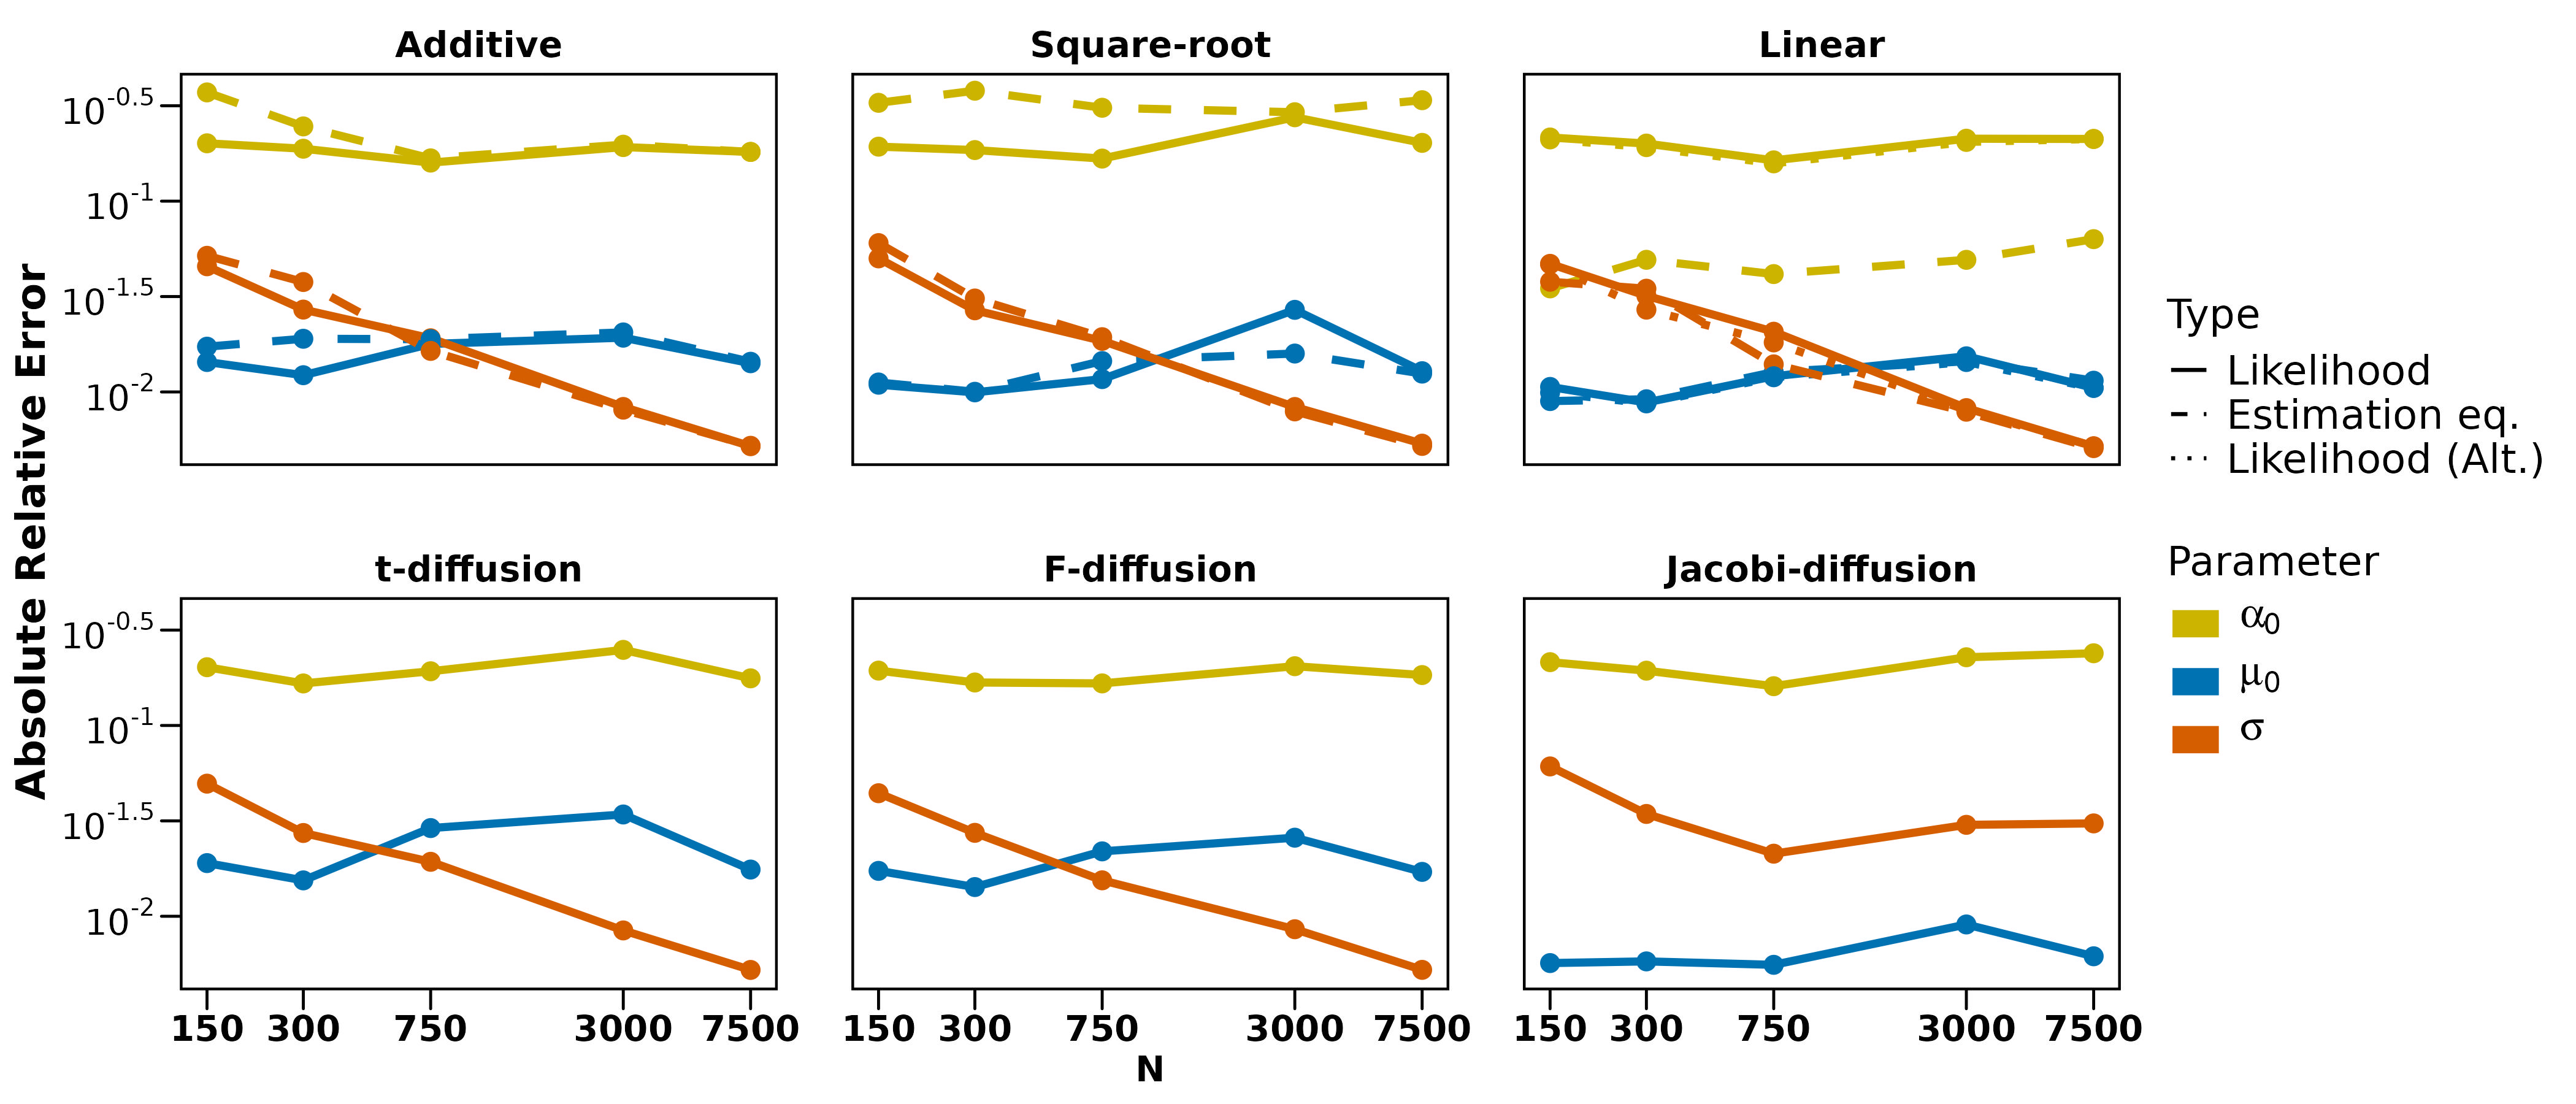
\includegraphics[scale = .1]{figures/parameter_precision_stationary.jpeg}
    \caption{Overview of our estimation methods for the stationary parameters applied to the models}
    \label{figure:overviewOfEstimatorsStationary}
    \end{center}
\end{figure}\\
Note that the specific scale this experiment is done at likely affects the results. The impression of the estimators here likely does not generalized. To see why this might be the case, consider for instance how noisy the additive model is in figure \ref{figure:samplesFromAllDifferentModels} compared to figure \ref{figure:samplesFromFiveDifferentModels}, and then recall that we are in the situation in figure \ref{figure:samplesFromAllDifferentModels}. On the other scale in figure \ref{figure:samplesFromFiveDifferentModels}, the parameters of the additive model might be relatively easier to estimate than the other models.\\
Moving on, we cleary see that the $\alpha_0$-parameter inherently is more difficult to estimate. Additionally, figure \ref{figure:overviewOfEstimatorsStationary} reveals that it is only really the $\sigma$ parameter for which more samples improve the absolute relative error; the other parameters mostly stay at their respective levels in terms of median ARE. The $\mu_0$-parameter is generally not very troublesome to estimate - for any model it consistently has an ARE of around $10^{-2}$, which is around 1.5 orders of magnitude lower than the $\alpha_0$-parameter. Still, all the parameters are relatively well estimated in median, indicating that they are quite robust even for starting values that deviates somewhat. Again, this might stem from the fact that the models could behave especially nicely on the unit interval.\\
For the models with more than one method there is no significant difference in the median ARE for $\mu_0$ and $\sigma$. With regards to $\alpha_0$, the alternative Strang method (\ref{meanrevertingGBMSplit1}) faired quite a bit better with an ARE of around an order of magnitude lower than the AOMEF and Strang method with the heuristic from \cite{SplittingSchemes}. To see how the models compare computationally, we consider the median computation time for the different methods as a function of $N$
\begin{figure}[h]
    \begin{center}
    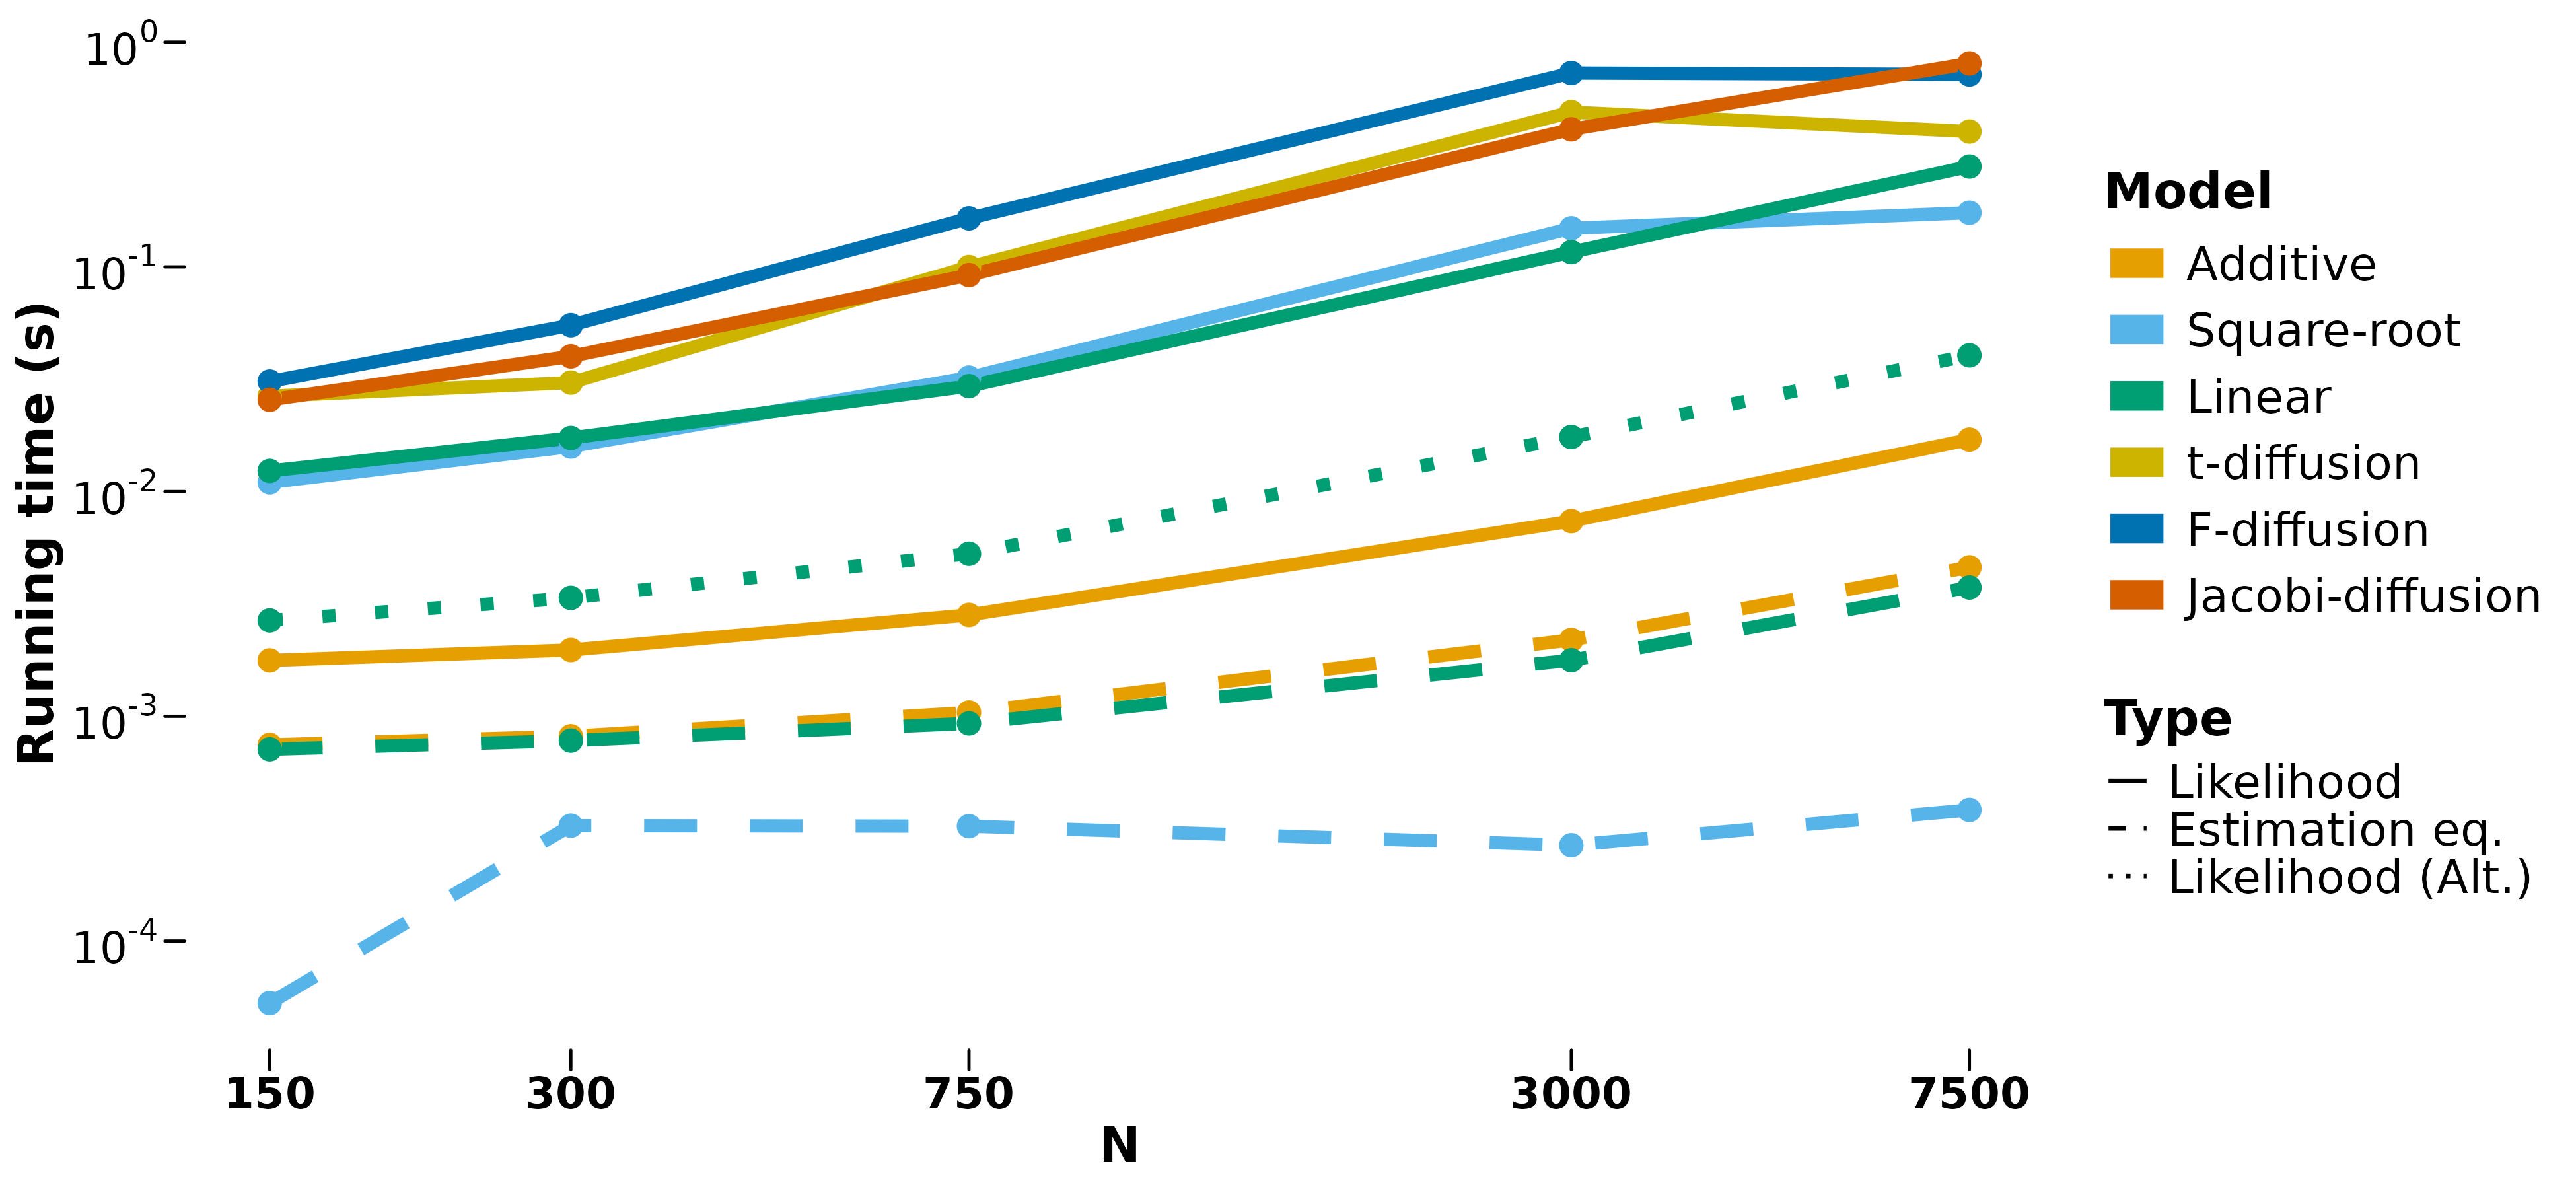
\includegraphics[scale = .075]{figures/estimation_duration_stationary.jpeg}
    \caption{Overview of our the median computation time for each method as a function of the number of samples}
    \label{figure:overviewOfDurationStationary}
    \end{center}
\end{figure}\\
This is the time from the invokation of the optimizer till the convergence criterion is reached. Generally, the estimation equations based estimators are much quicker than the likelihood based, but the explicit estimators based on (\ref{eq:squarerootMartingaleEquation}) for the square-root diffusion are naturally in a league of it owns being between 100 and 1000 times quicker than the likelihood based methods. The latter are generally in the same order of magnitude in terms of performance. Though, the $F$-, $t$- and Jacobi-diffusion based models are slower than the linear and square-root based models. This might be caused by the more complicated ordinary differential equations in these models, which the Runge-kutta needs to solve repeatedly; compare the expression in (\ref{eq:squarerootStationarySplit2}) and (\ref{eq:GBM_StrangNonLinearODE_split}) with (\ref{eq:StrangTDiffusion}), (\ref{eq:FscaledSplitting}) and (\ref{eq:jacobiODE}). If we look at the likelihood based methods that solves the ordinary differential equations numerically and contrast their computation time with the ones that are either use MLE or has a closed form solution to the ODE (\ref{meanrevertingGBMSplit1}), it is clear that there is a computational cost to solving the ODE numerically.
\subsubsection{The dynamic parts}
Turning to investigating the estimation in the dynamic part of each model, recall that we only use variations of the Strang-method for this. If more than one is used, it is denoted \textit{Strang (Alt.)} here. The alternative Strang estimators are the ones not based on the heuristic in \cite{SplittingSchemes}, i.e. the two estimators based on (\ref{eq:squareRootSplit2}) and (\ref{eq:GBMSplit2}) used in the square-root- and Linear models, respectively. We simulate from the models and fit in the manner described above. The ARE of the parameters in the dynamic part is depicted as a funtion of $N$ using a double logarithmic scale 
\begin{figure}[h!]
    \begin{center}
    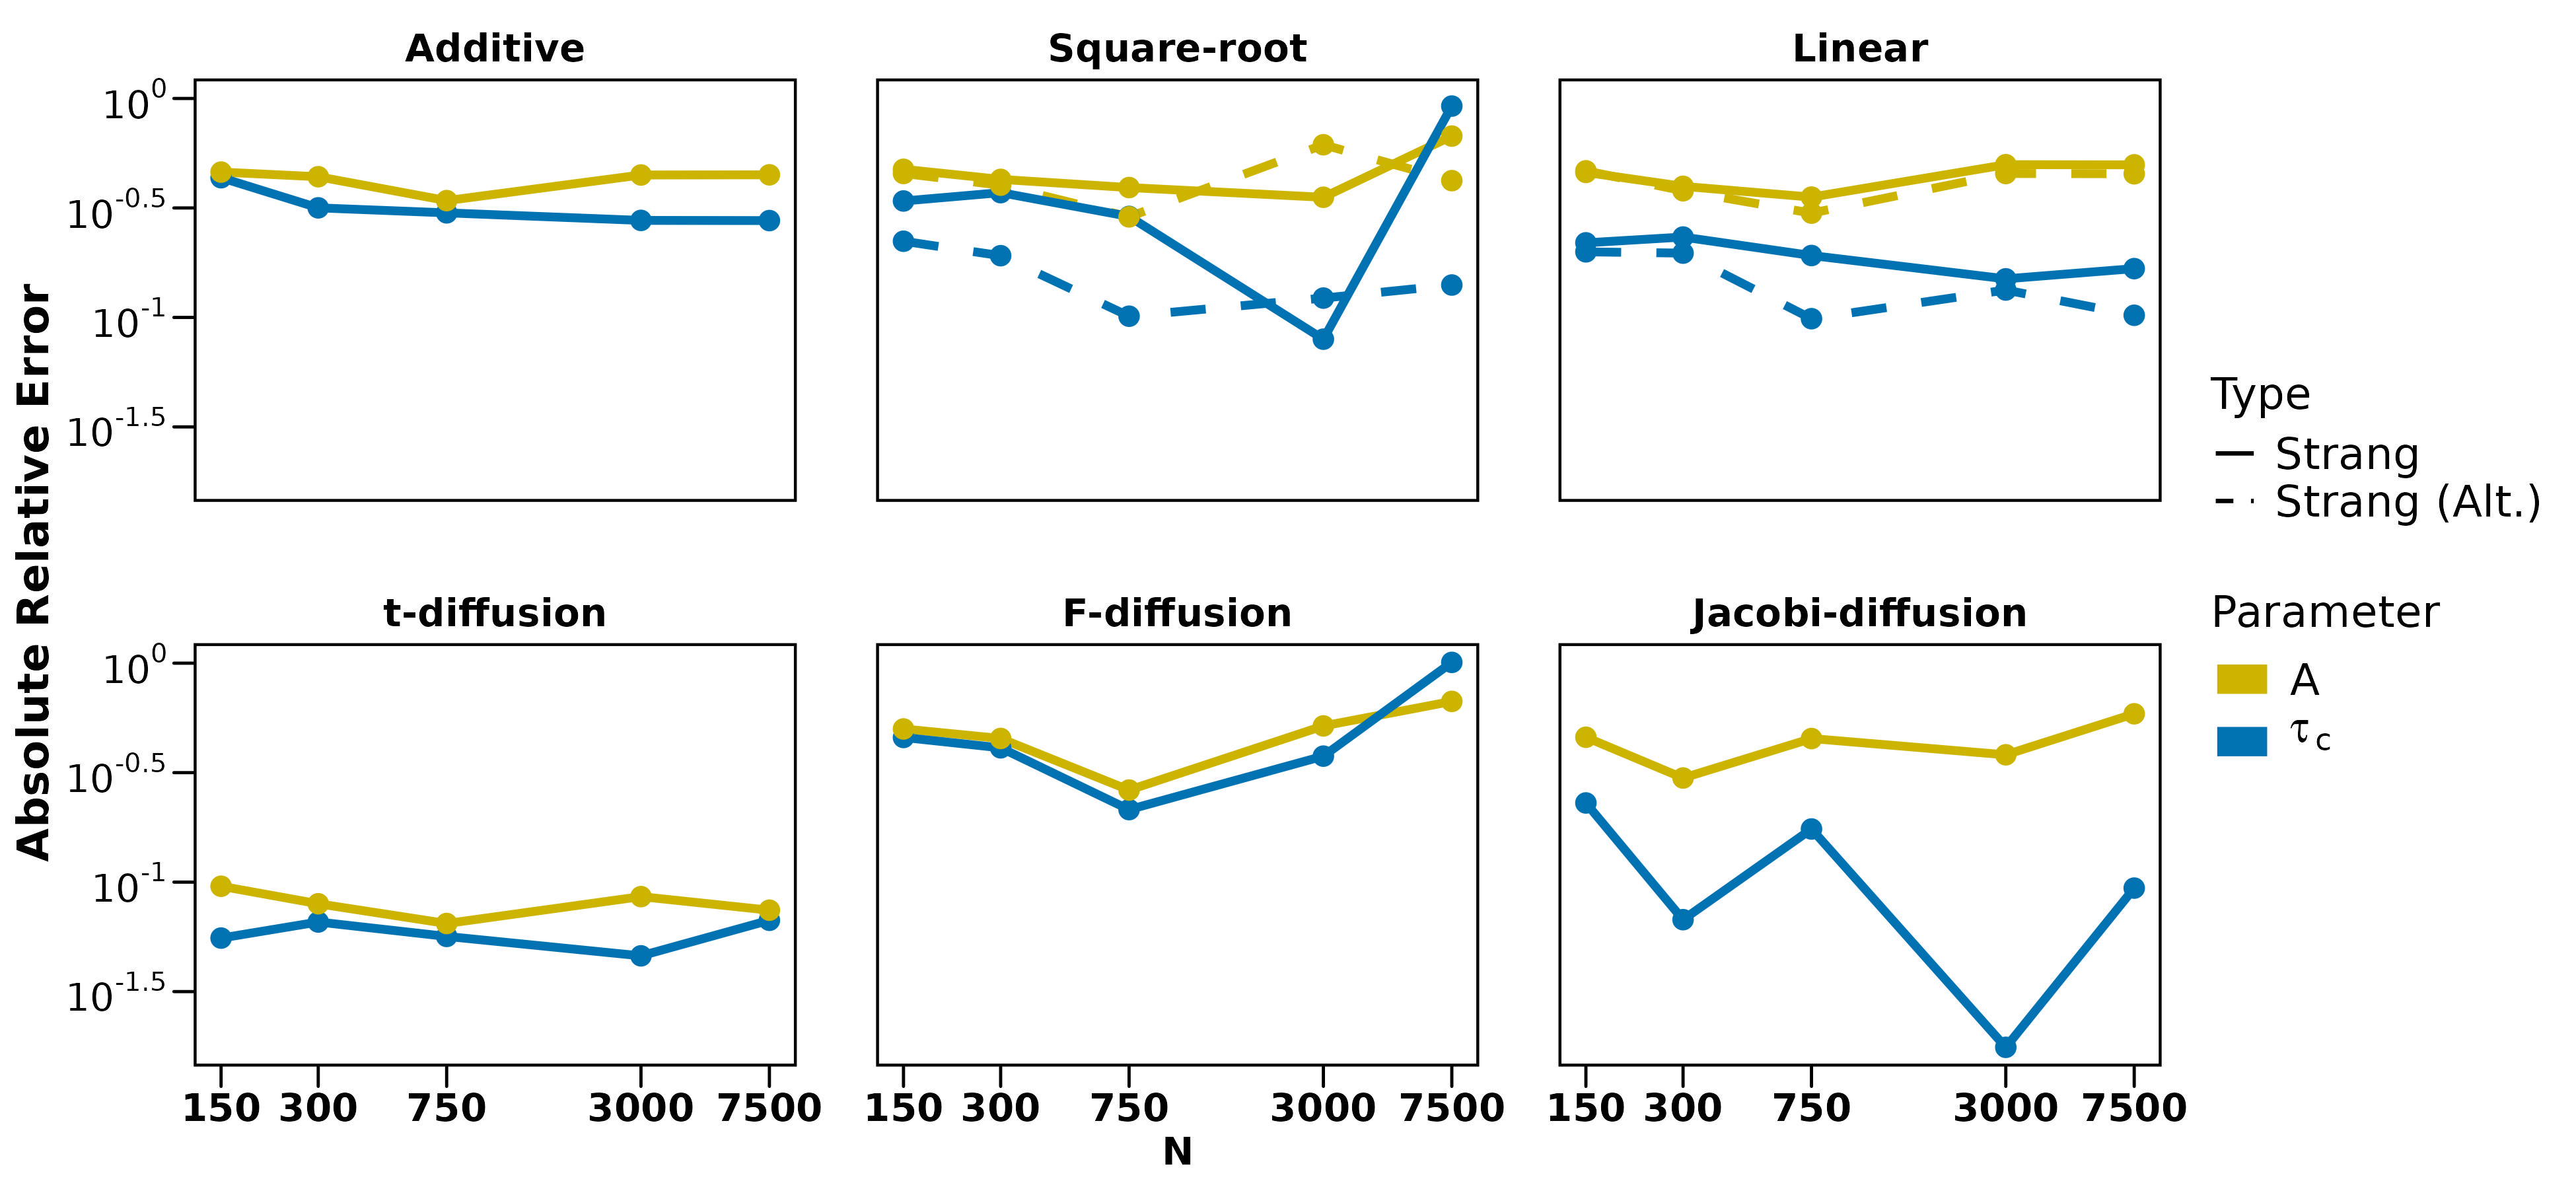
\includegraphics[scale = .1]{figures/parameter_precision_dynamic.jpeg}
    \caption{ARE of the parameters of the models in the dynamic part}
    \label{figure:parameter_precision_dynamic}        
\end{center}
\end{figure}\\
It is generally much harder to estimate in the dynamic part. In terms of the $A$-parameter all models and type of methods faired relatively equally in terms of ARE. That is with the exception of the $t$-diffusion model, whose ARE are around half an order of magnitude smaller than that of the mother models. For some reason, the normal Strang estimator in the Square-root model as well as the $F$-diffusion based model show a relatively high median ARE for the largest number of samples we investigated.  Considering the other sample sizes this is more surprising for the Square-root noise model, as it is generally easier to estimate in. The $F$-diffusion seems, on this scale at least, to be the hardest of the models to do estimation on; whereas, as we mentioned, the $t$-diffusion based model seems the easiest. In terms of overall run time, we achieved similar results in terms of which kinds of models had faster convergence as we saw in figure \ref{figure:overviewOfDurationStationary}. For this reason, the results are only shown in appendix \ref{section:benchmark} in figure \ref{figure:estimation_duration_dynamic}. One surprise from this benchmark though, is the fact that $t$-diffusion based model, which solves its ODE numerically, has the fastest convergence of all the models. This probably stem from the model requiring less iterations overall before convergence is reached, as solving the ODE with Runge-kutta is much more computationally expensive than just computing the solution.

\subsection{Fitting the $\nu$-parameter}
We now consider how introducing the $\nu$-parameter into the model affects the performance of the optimizers. For simplicity, we focus on the additive- and t-diffusion based models in this experiment. We ensure that the Brownian motions in a specific run in the simulation are the same. We simulate from both models using $t_0 = 54$ and $\tau_c = 132$ and temporal resolutions $\Delta t = \{1/3, 1/5, 1/25, 1/50, 1/100\}$, which correspond to $N_\mathrm{dynamic} = \{396, 660, 3300, 6600, 13200\}$ samples in the dynamic part. The dynamic part is the important one here, because this is where $\nu$ is estimated. The other parameters are $\theta = (0.87, -1.51, -3,  0.387)^\top$. Estimation is also done in the stationary part, but this is only used to pass onto the optimizers in the dynamic parts. For this reason, optimization here is initialized in the true stationary parameters. In the dynamic part optimization is initialized in a similar manner to earlier experiments. We add $\pm 10\%$ multiplicative noise to the true values of $A$ and $\tau$ by sampling two uniform variables according to $U\sim \mathrm{Unif}(0.9,1.1)$. The last parameter $\nu$ is always started in $1$, regardless of the true value. This is done to simulate the user assuming the more parsimonious with $\nu = 1$ and then letting the data show that $\nu$ is something else. For each value of $\Delta t$ we investigate how the models and optimizers perform on $\nu_{\mathrm{sim}} = \{0.75, 0.9, 1, 1.11, 1.33\}$. For each combination we run $M = 50$ simulations. As earlier, we consider the median of the ARE for each combination of $\Delta t$ and $\nu$. The experiments are once more implemented such that failure to convergence or run the optimization results in a graceful exit. Now, instead of merely retrying after a failed optimization attempt, we count how many time each model fails for every combination of $\Delta t$ and $\nu$. This is to highlight, if there is a specific model or parameter value of $\nu$ that is troublesome to estimate on. The relative tolerance convergence criterion in \code{optim} was set to \code{sqrt(.Machine\$double.eps) / 1000} to avoid getting stuck in local minima. 
We start by considering the ARE 
\begin{figure}[h!]
    \begin{center}
        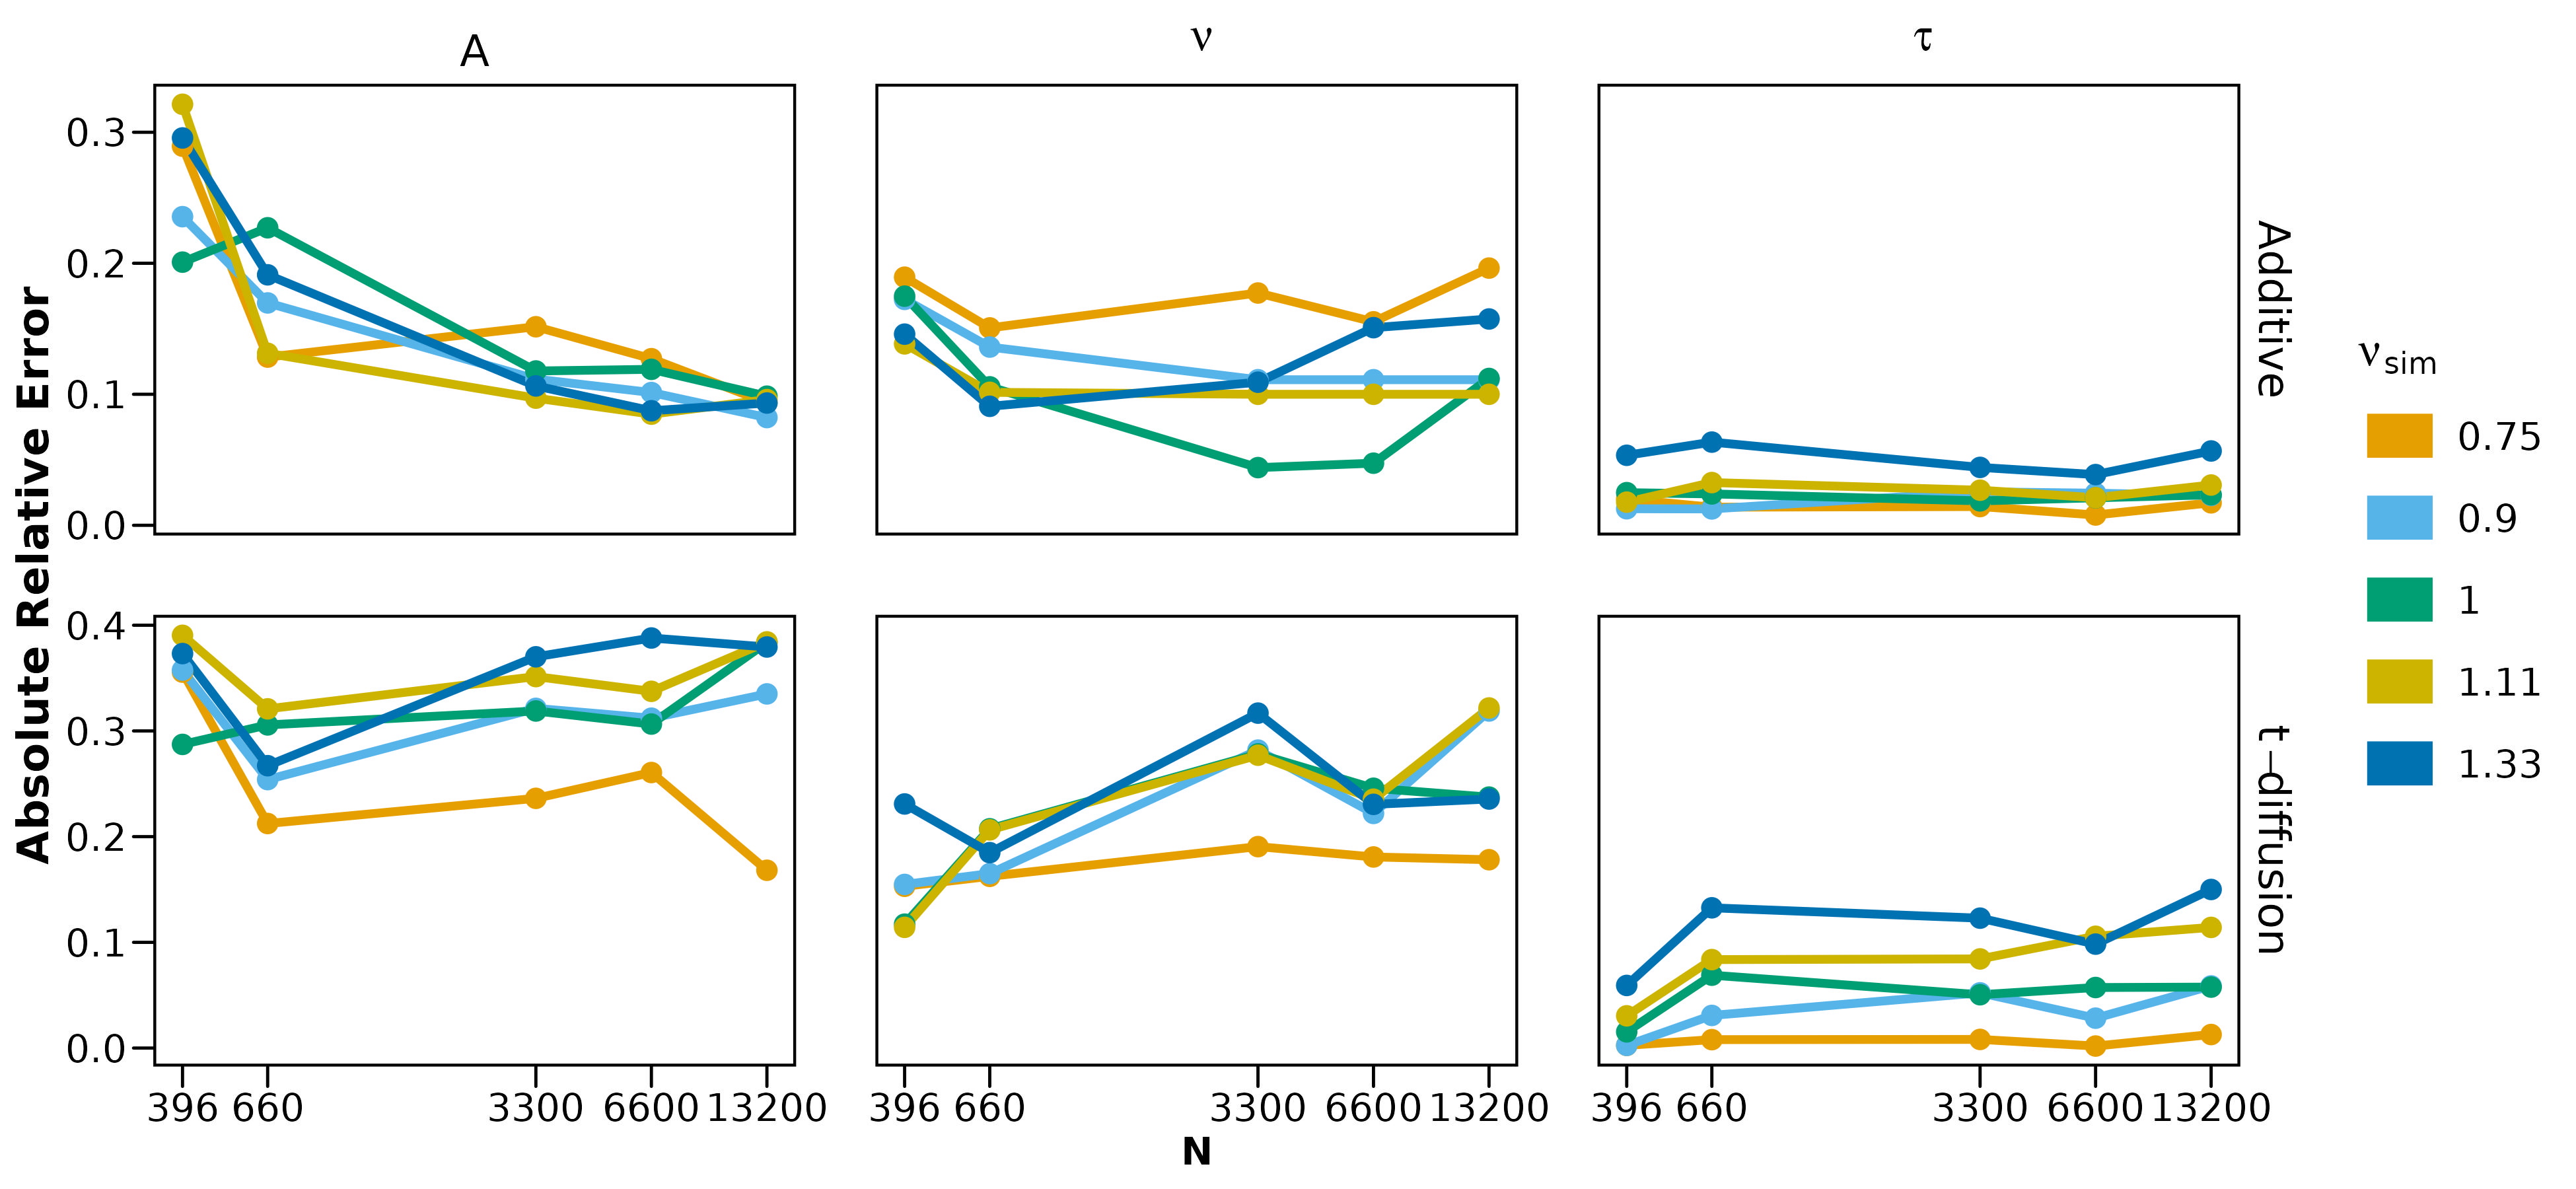
\includegraphics[scale = .1]{figures/combined_nus_plot.jpeg}
        \caption{The absolute relative error of the different parameters as a function of $N$ for diffferent true values of $\nu$.}
        \label{figure:ARE_nu_plots}
    \end{center}
\end{figure}\\
Note that the $x$-axis is logarithmic in figure \ref{figure:ARE_nu_plots}. From the graph we see that increasing the number of samples only really makes the median ARE better for the model with additive noise and only considerably for the $A$-parameter. Though, the median ARE for the other parameters are generally low. Increasing the true value of the $\nu$-parameter, does result in an overall larger ARE. If we look at figure \ref{figure:nu_plot}, this is not too surprising. As we commented, an increase in $\nu$ results in the two fixed points being closer to one another longer before the bifurcation point. This creates a situation, where the process tips due to noise more frequently - thus making it difficult to estimate when bifurcation tipping would occur. All in all, though, the values depicted here does not seem to alarming considering the added flexibility having a $\nu$-parameter provides. However, we also counted how many times each method failed during optimization - this yielded the following results
\begin{figure}[h!]
    \begin{center}
        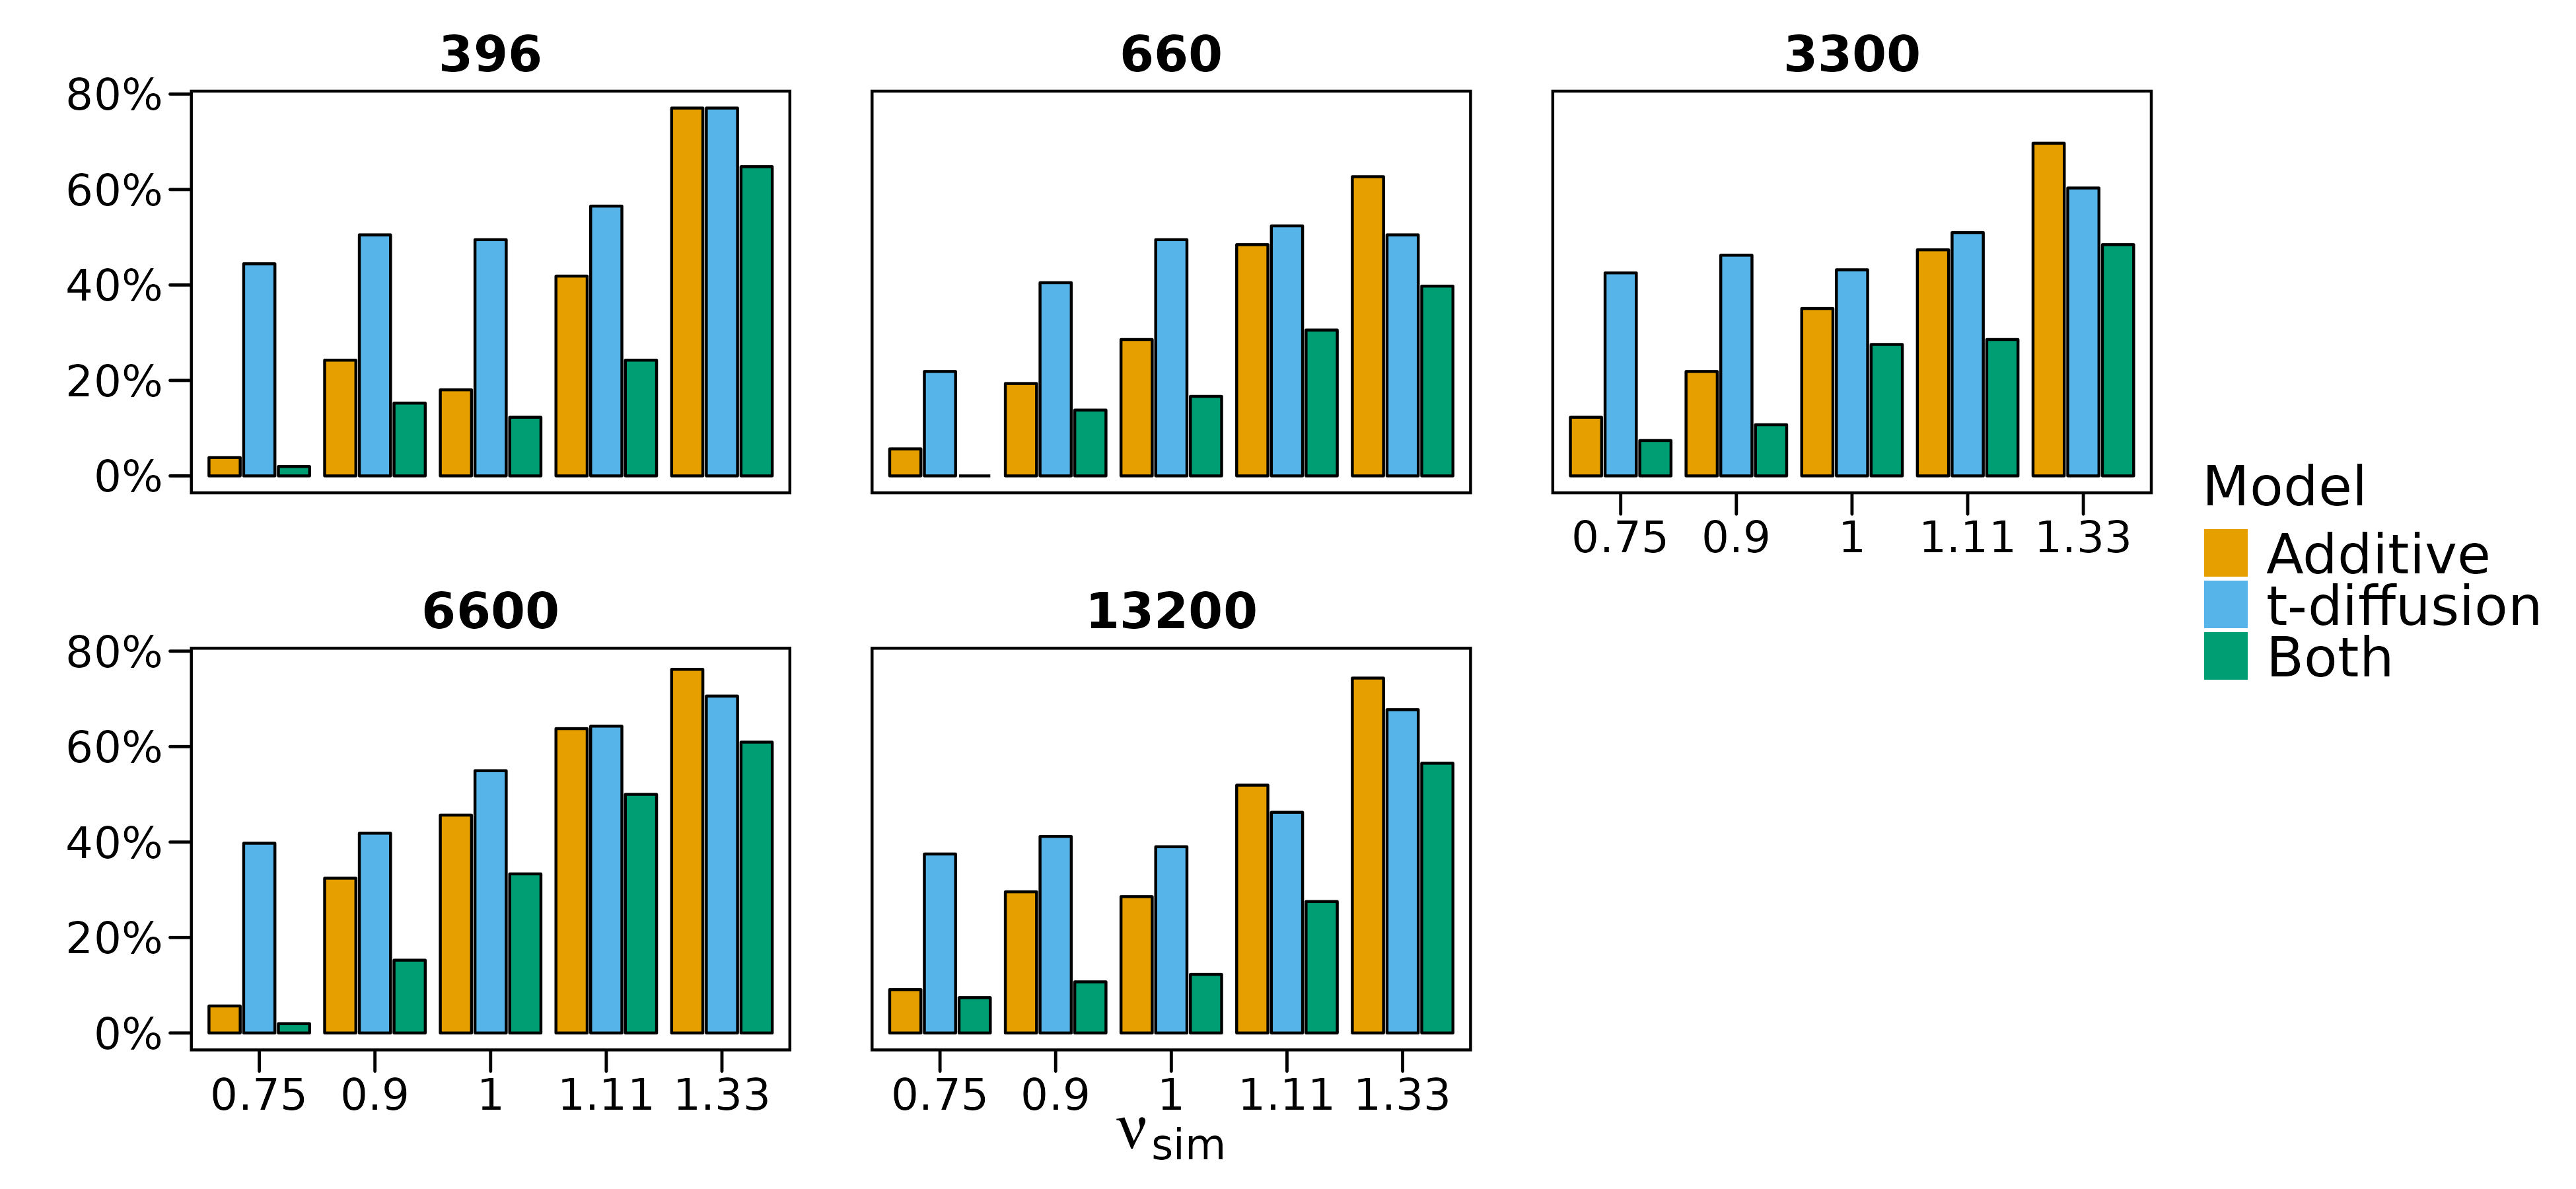
\includegraphics[scale = .1]{figures/error_count_plot.jpeg}
        \caption{The proportion of times where the respective models or both failed doing optimization as a function of $N$ and for different true values of $\nu$.}
        \label{figure:error_count_nu_experiment}
    \end{center}
\end{figure}
Keep in mind that the $x$-axis is now $\nu_{\mathrm{sim}}$, whereas the individual elements in the grid correspond to graphs for different values of $N$. Evidently, estimating with $\nu$ in the model estimation fails quite frequently. This is even when we a provided with estimates from the stationary part, where optimization was initialized in the true values. In comparison, the methods virtually never fail to optimize, when we only opt for estimation of $A$ and $\tau_c$ in the dynamic part. Now, the model with additive noise faires better overall and it seems that as long as the true value $\nu\leq 1$ the is a reasonable chance of success with it. The model does not seem to become better for larger sample sizes unfortunately. Conversely, the $t$-diffusion based model has for all samples sizes at least a $20\%$ chance of failing, which is unacceptable. From the green bar it is also rather clear that whenever the additive models does fail, it is often the case that the $t$-diffsion based model fails as well.  
\subsection{Early warning analysis}

\subsection{The numerical Strang}
We introduced the idea of the numerical Strang splitting in section \ref{subsection:NumericalStrangSplitting}. In sum, the aim was to numerically do as many of the computations to make a Strang splitting scheme that follows the heuristic in \cite{SplittingSchemes} as possible. The implementation we ended up with only needed to be provided the lamperti transform and the drift of the Lamperti-transformed SDE, and then it would take care finding fixed points, constructing the linear SDE etc. In this section, we constrast the numerical Strang applied to two models with their respective analytical counterparts. The ones we consider are the model with linear noise and the F-diffusion based model. \\These models have their ODE solved numerically, meaning that the terms "analytical" and "numerical" should be understood relatively. For clarity we will instead refer to the "analytical" method as \textit{closed-form} alluding to the fact that it is the one where we use the closed form solution of the fixed point. For their lamperti-transform confer table \ref{table:ergodicDiffusions}, while the lamperti drifts can be found at (\ref{eq:GBM_lamperti}) and \ref{eq:F_diffusion_lamperti_SDE}. Because of the time dependence of the fixed points through $\lambda_t$ in the dynamic parts, we did not consider these, as it would be much more difficult to implement a method that finds a fixed point for each time-point in a process. We simulate using $A = 1.5$, $m=0.4$, $\lambda_0 = -0.2$ and $\sigma =0.15$ as well as $t_0 = 30$ with temporal resolution $\Delta t = \{1/5, 1/50, 1/150, 1/500, 1/1000\}$, in other words: $N =  \{150, 1500, 4500, 15000, 30000\}$.  The parameters correspond to $\alpha_0 = 1.095$, $\mu_0 = 0.7651$ and $\sigma = 0.15$ for the true parameters of the stationary part; these are the parameters we want to estimate. For each value of $N$, we run $M = 50$ simulations, do estimation and time the estimation with \code{microbenchmark}. Optimization is initialized at noisy starting values as previously. This time the uniform variables are samples such that each coordinate has a deviation from the true value of up to $\pm 25\%$ at random; though as before this noise is the same for all methods in a specific run of the simulation. We let the methods fail gracefully, but again keep track of how many time each method fails. Apart from this metric, we consider the distribution of the ARE to get a detailed view of how the methdods perform - also in the extreme case. Here, the results are shown for the model with linear noise as our findings are the most clear in this model. Still, the same results as we are about to show, can be found for the $F$-diffusion based model in figure \ref{figure:ARE_dist_numeric_F_diffusion} in appendix \ref{section:benchmark}. \\For the linear model, though
\begin{figure}[h!]
\begin{center}
    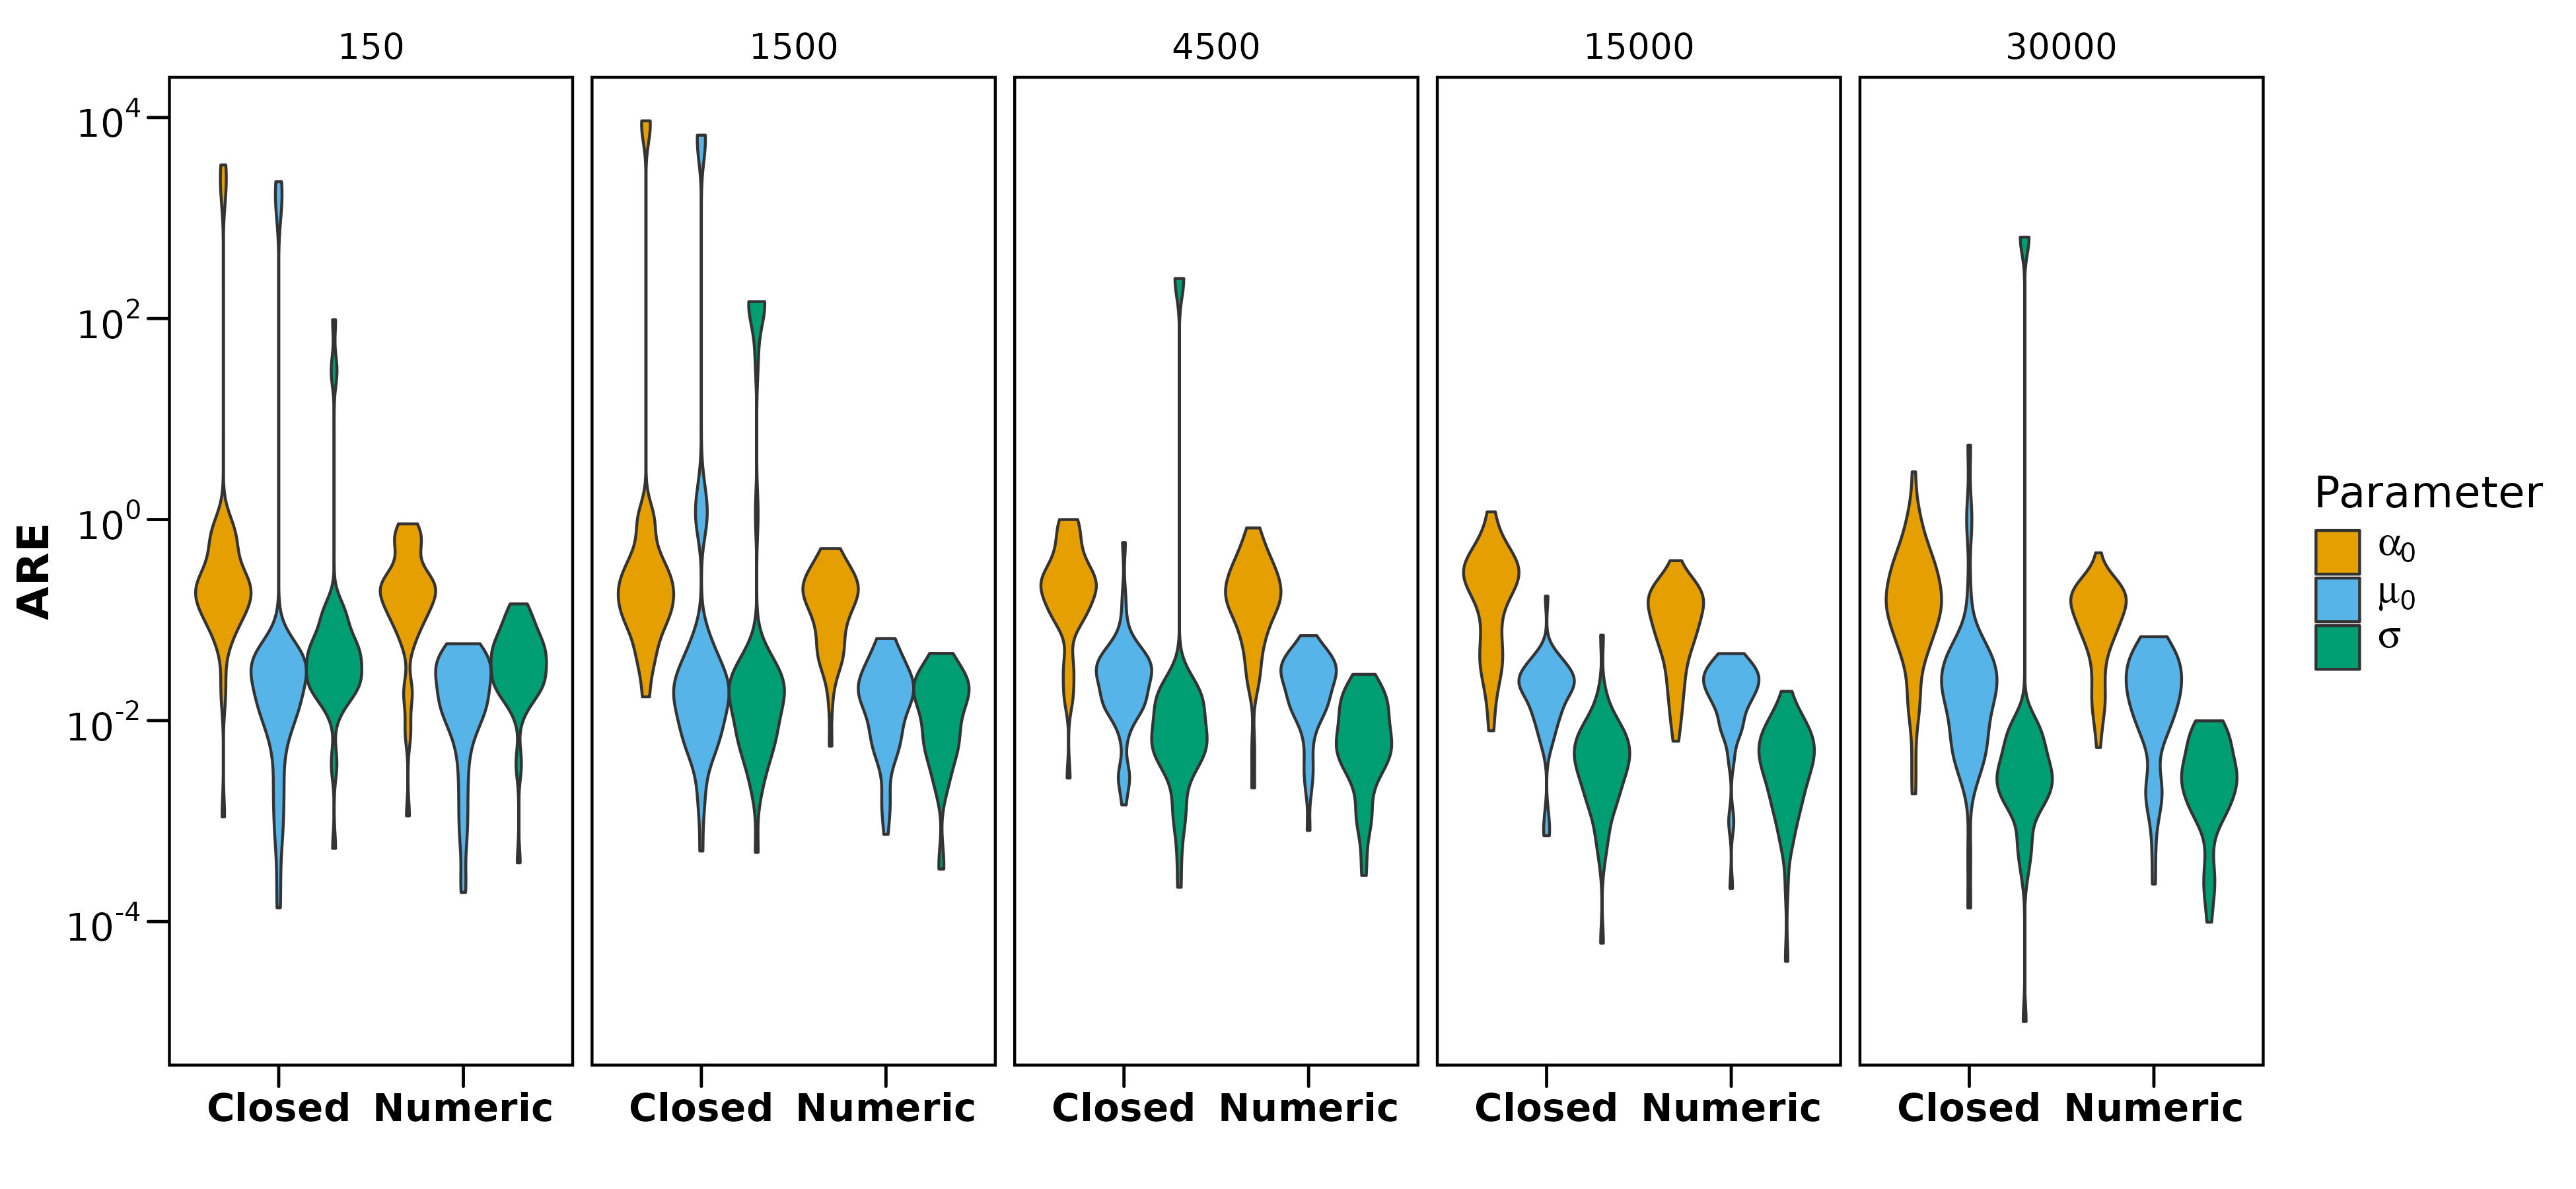
\includegraphics[scale = .1]{figures/ARE_dist_result_plot_Linear.jpeg}
    \caption{Distribution of the ARE of the parameters in the linear noise based model shown for the numeric and closed form type estimation methds.}
    \label{figure:ARE_dist_linear_noise}
\end{center}
\end{figure}\\
Initially, it is worth mentioning that across all runs in both models, it was only the closed form solution of the linear-model that ever fail to optimize. It did this around $20\%$ of the time for $N = 150$; $2\%$ for $N = 4500$ and $4\%$ for $N = 30000$, but never at other $N$. This fact aligns well with the results depicted in figure \ref{figure:ARE_dist_linear_noise} as it suggests a lack of overall robustness of the method. In the graph we see that there are a few quite extreme ARE-observations for parameters estimated by the closed form method. Conversely, a general better performance of the numeric estimator is evident by the fact that the distribution of the ARE for a specific parameter and fixed number of samples is shifted towards zero for this estimator.  
\subsection{Model misspecification}
